%%%%%%%%%%%%%%%%%%%%%%%%%%%%%%%%%%%%%%%%%%%%%%%%%%%%%%%%%%
%%%%%%%%%%%%%%%%%%%%%%  Question#02  %%%%%%%%%%%%%%%%%%%%%
%%%%%%%%%%%%%%%%%%%%%%%%%%%%%%%%%%%%%%%%%%%%%%%%%%%%%%%%%%
\begin{comment}
  Put all the topics for this question.
\end{comment}
%%%%%%%%%%%%%%%%%%%%%%%%%%%%%%%%%%%%%%%%%%%%%%%%%%%%%%%%%%
\question 
\begin{parts}
%%%%%%%%%%%%%%%%%%%%%%%%%%%%%%%%%%%%%%%%%%%%%%%%%%%%%%%%%%	
\part[2] For units, you can use SI unit, \textcolor{blue}{as for example} \textcolor{red}{\SI{2}{\micro\meter}} can be achieved by using the command \verb|\SI{2}{\micro\meter}|. In case you need to use the unit for an expression \textcolor{blue}{as for example} \textcolor{red}{ \(20sin(\omega t)\)~\si{\milli\ampere}}, right after the expression, you can use the command \verb|\si{\milli\ampere}|.


\begin{solution}

\end{solution}
%%%%%%%%%%%%%%%%%%%%%%%%%%%%%%%%%%%%%%%%%%%%%%%%%%%%%%%%%%
\part[4] Two resistors of values \SI{1}{\kilo\ohm} and \SI{4}{\kilo\ohm} are connected in series across a constant voltage supply of \SI{100}{\volt}. A voltmeter having an internal resistance of \SI{12}{\kilo\ohm} is connected across the \SI{4}{\kilo\ohm} resistor. Draw the circuit and calculate: 

\begin{subparts}
		\subpart True voltage across \SI{4}{\kilo\ohm} resistor before the voltmeter was connected.
		\subpart Actual voltage across \SI{4}{\kilo\ohm} resistor after the voltmeter is connected and voltage recorded by the voltmeter.
		\subpart change in supply current when voltmeter is connected.
		\subpart Percentage error in voltage across \SI{4}{\kilo\ohm} resistor.
	
	\end{subparts}



\begin{solution}

\end{solution}
%%%%%%%%%%%%%%%%%%%%%%%%%%%%%%%%%%%%%%%%%%%%%%%%%%%%%%%%%%	
\part[5] \color{red}If you want to insert a Figure(pdf, png, etc) then you can use the \verb|\includegraphics{nameOfFigure}| command as shown below. : \color{black}Find the rms value of the current waveform of Fig.\ref{fig:currentWaveform}. If the current flows through a \SI{9}{\ohm} resistor, calculate the average power absorbed by the resistor. 


		\begin{figure}[H]
			 \centering 
			 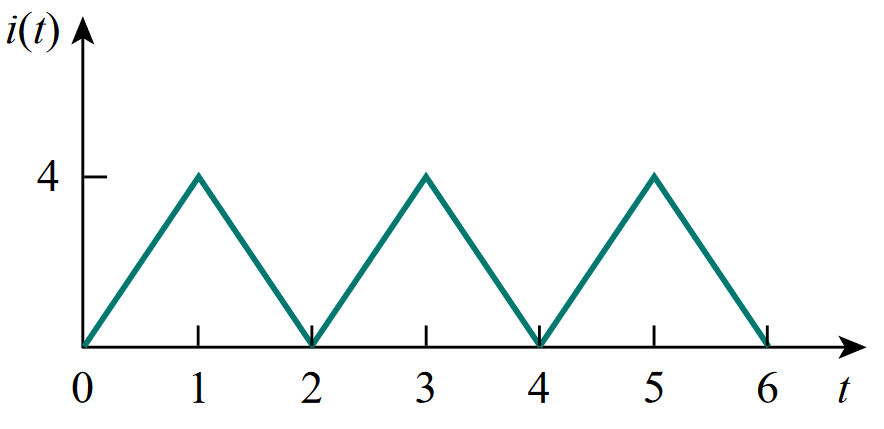
\includegraphics[width=0.4\textwidth]{Fig11.15_ElectricCircuit_SadikuPg446_3E}
			 \caption{}
             \label{fig:currentWaveform}
        \end{figure}
		


\begin{solution}

\end{solution}
%%%%%%%%%%%%%%%%%%%%%%%%%%%%%%%%%%%%%%%%%%%%%%%%%%%%%%%%%%			
\end{parts}

